\chapter{Tipos de processos de produção industrial}
\label{chap:tipos_de_processo_de_producao}

Nesta seção será discutido a classificação dos diversos tipos de empresas industriais partindo de seus processos de produção. Esta tarefa é importante na concepção de novas instalações industriais, pois permite identificar e reconhecer as características básicas da empresa industrial, a partir de seu processo produtivo. Por fim, na seção \ref{sec:tipos_de_processo_de_producao_aplicacao} será mostrado a aplicação prática referente ao tipo de processo adotado pela \textit{SunBurn}.

\section{Sec1}
\label{sec:tipos_de_processo_de_producao_sec1}

As unidades produtivas podem variar desde o volume de produção (alto, médio ou baixo) até a variedade de seus produtos (alta, média ou baixa). Por isso, pode se dizer que as variáveis volume e variedade são dependentes entre si, por exemplo, operações de alto volume em geral têm baixa variedade de produtos e vice-versa. Portanto, existe uma relação inversa entre o volume e a variedade do produto \cite{slack2009administracao}.

A figura \ref{fig:tipos_de_processo_de_producao} nos mostra como os cinco tipos de processos existentes estão arranjados de acordo espectro variedade-volume. Além disso, as características de cada um destes processos serão descritos, com base no volume e variedade, descendo pela diagonal que parte do canto superior esquerdo até canto inferior direito. Em outras palavras, os processos serão descritos a seguir partindo das empresas com uma maior variedade e baixo volume até uma baixa variedade e alto volume.

\begin{figure}[H]
  \caption{Matiz Variedade x Volume: Definindo os cinco tipos de processos produtivos ALTERAR A IMAGEM E O TITULO}
  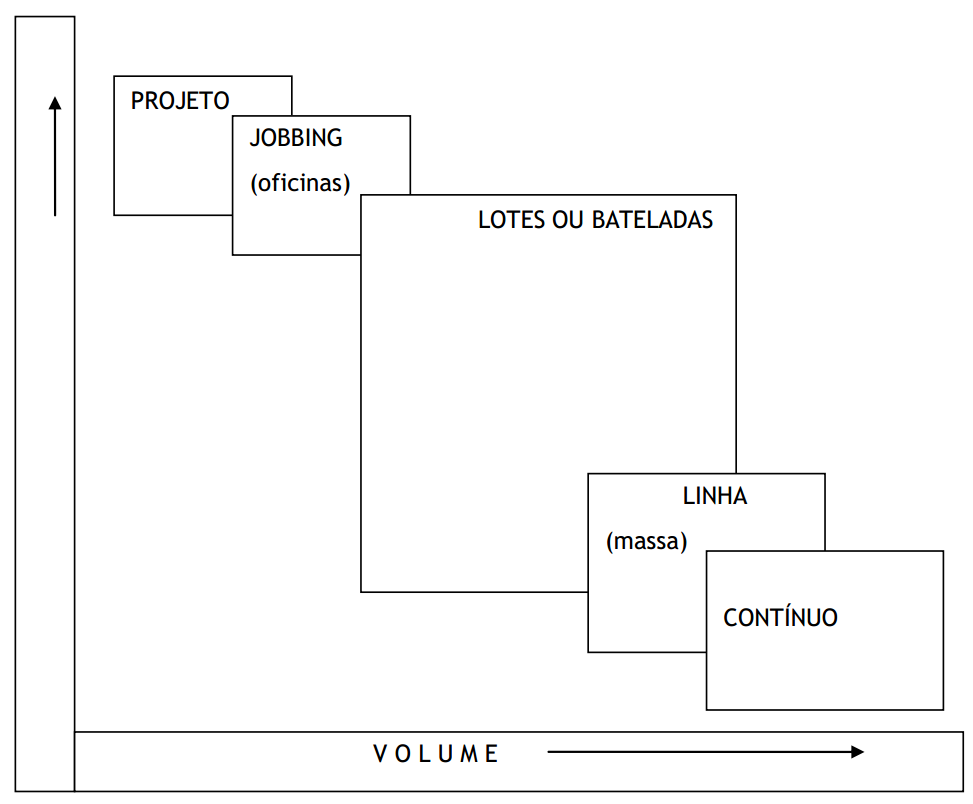
\includegraphics[scale=0.5]{images/tiposdeprocesso.png}
  \caption*{Fonte: Adptado de \cite{slack2009administracao}}
  \label{fig:tipos_de_processo_de_producao}
\end{figure}

O processo de projeto é carecterizado por ....

\section{Aplicação Prática}
\label{sec:tipos_de_processo_de_producao_aplicacao}